\section{Formalisation}
\label{sec:Formalisation}
\moussa{Rewrite this descripton}

Our formalisation defines a \emph{paradigm} as a set of 
\emph{characterising properties} $\mathsf{\Pi}$ that holds over a mathematical 
construction called a \emph{paradigmatic structure} $\mathsf{PS}\in \PS$. 
This structure describes a specific \emph{workflow} (or \emph{process}) that 
captures how specific \emph{languages instances} are combined together, 
through transformations, towards achieving a specific intent $\iota$ that is 
adequately characterised by the properties. When $\iota$ has a commonly agreed 
name (in a given context, or for a specific community), and $\mathsf{\Pi}$ holds 
on a specific $\mathsf{PS}$, then $\mathsf{PS}$ is said to \emph{qualify} as 
the paradigm $\iota$. The properties constituting $\mathsf{\Pi}$ may 
characterise the formalisms and/or the workflow defining a paradigmatic 
structure. 

\arend{Annotate the rest of this section to improve definitions, and formalisation as coherent as possible.}

%%%%%%%%%%%%%%%%%%%%%%%%%%%%%%%%%%%%%%%%%%%%%%%%%%%%%%%%%%%%%%%%%%%%%%%%%%%%
% \subsection{Preliminaries}
% \label{sec:Formalisation-Preliminaries}
% 
% \begin{olddef}
% We assume in this paper that ``\emph{everything is modelled explicitly}`` by 
% using \emph{models} conformant to \emph{metamodels}, themselves explicitly 
% modelled (using a \emph{meta-metamodel}). The following definition introduces 
% precise notations for these notions.
% 
% \begin{Definition}[\label{def:MMM}(Meta-)Models \& Conformance]
%    Let $\mathbb{M}$ and $\mathcal{M}$ be the sets of all models and metamodels 
% respectively, as defined by meta-metamodels. For a model $\mathsf{M} \in 
% \mathbb{M}$ and a metamodel $\mathsf{MM} \in \mathcal{M}$, we write $\mathsf{M} 
% \rhd \mathsf{MM}$ if $\mathsf{M}$ \emph{conforms to} $\mathsf{MM}$.
% \end{Definition}
% This definition explicitly distinguishes between two meanings for what is 
% called an \emph{instance}, namely the difference between \emph{linguistic} and 
% \emph{ontological} instantiation \cite{J:Kuhne:2006}. \textsf{M} and \textsf{MM} 
% are \emph{valid} (linguistic) instances of their respective meta-metamodels in 
% the sense that they belong to the valid ''\emph{phrases}'' that the 
% meta-metamodel defines; whereas the fact that \textsf{M} is an 
% \emph{ontological} instance of \textsf{MM} needs to be checked, making 
% \textsf{M} conform to \emph{MM}. This checking procedure has been extensively 
% described by many previous contributions (see e.g. 
% \cite{PhD:Amrani:2013,J:Rivera-Duran-Vallecillo:2009}).
% \end{olddef}
% \begin{newdef}
% In this paper we follow the motto that ``\emph{everything is modelled explicitly}''. This means that, whenever we have a set of things we want to reason about (models, transformations, properties) we specify that set in some concrete fashion. The set is then called the \emph{extension} and its specification its \emph{intension}. A given object is said to \emph{conform} to a specification if it is an element of its extension. Checking conformance can be a non-trivial task in practice.
% 
% In many contexts, the intension is called a \emph{metamodel} and an element of its extension a \emph{model}. Metamodels themselves also form a set, and so according our own motto can be specified in a \emph{meta-metamodel}. 
% \end{newdef}
% 
% The choice of a specific meta-metamodel determines the technological space 
% chosen for metamodelling \cite{Wimmer-Kramler:2005}: \emph{grammarware} have a 
% tree-based structure and are fully textual; whereas \emph{modelsware} are either 
% visual or textual (or both), and rely either on \textsc{Mof}-like tree-based 
% (meta-)metamodels, or Graph Theory. 
% 
% 
% % Take as a simple example \emph{object orientation} as a fairly recognised 
% % intent, which may translate into the following list of properties: the 
% % existence of objects possessing an identity; a notion of class that types 
% % objects, and that defines data and functions of these objects; a relation on 
% % classes called inheritence that allows objects of one class to acquire 
% % properties of objects of another class; and the existence of a message passing 
% % mechanism between objects. 
% % \moussa{Maybe factor out this description in a previous section dedicated to 
% % provide the intuition about paradigms?}. 
% 
% \begin{olddef}
% In order to designate specific items of our formalisation explicitly by their 
% name, we define distinct namespaces as sorted sets. Properly resolving 
% namespaces is out of scope, as it relies on specific tooling 
% capabilities and implementation choices.
% 
% \begin{Definition}[Names]
%    The sorted set $\mathsf{Name}$ of \emph{names} defines namespaces over 
% \emph{items}.
%    \begin{small}
%    \begin{displaymath}
%      \begin{array}{rcl}
% 		\mathsf{Item} & \eqdef & \{\mathsf{AbstractFormalism}, \mathsf{Language}, 
% \mathsf{Transformation}\\
%                     &        & \mathsf{Intent}, \mathsf{LangInstance}, 
% \mathsf{TransInstance}\}\\
% 		\mathsf{Name}    & \eqdef & (\mathsf{Name}_{_{\mathsf{e}}})_{_{\mathsf{e} 
% \in \mathsf{Item}}}
%       \end{array}
% \end{displaymath}
%    \end{small}
% \end{Definition}
% To avoid the subscripted notation, we introduce a more compact notation for 
% referring to names: for example, the set of class names 
% $\mathsf{Name_{_{Language}}}$ will be noted $\mathsf{LanguageN}$.  
% \end{olddef}
% \begin{newdef}
% In order to be able to refer to elements of our formalisation, we introduce the concept of \emph{names}, which are \emph{identifiers} in a \emph{namespace}. Namespaces are themselves either also names, or can be the top (global) namespace. To formalise this, we assume a universe of \emph{identifiers} $\ID$, and a \emph{top namespace} $\top$; then the set of namespaces \NS and the set of names \Name are the smallest sets satisfying
% \[\begin{array}{rcl}
% \NS & \eqdef & \{\top\} \cup \Name \\
% \Name & \eqdef & \NS \times \ID
% \end{array}\]
% We immediately adopt the common dot-separated (concrete) syntax for names.
% For instance, \textsf{ANSI.C} denotes the name $((\top,\mathsf{ANSI}), \mathsf{C})$: it is the qualified name of the language with identifier \textsf{C} in the namespace \textsf{ANSI}, which is itself a name consisting of the identifier \textsf{ANSI} in the top namespace, $\top$. Another example of a namespace is this paper itself: the terminology used in this paper should be understood in that namespace --- we are well aware that the same identifiers (such as \textit{language}, \textit{formalism}, \textit{syntax}) can and do have different definitions elsewhere.
% \end{newdef}

%%%%%%%%%%%%%%%%%%%%%%%%%%%%%%%%%%%%%%%%%%%%%%%%%%%%%%%%%%%%%%%%%%%%%%%%%%%%
% \subsection{Formalism \& Language}
% \label{sec:Formalism-Language}
% 
% \begin{olddef}
% We first introduce a distinction between \emph{formalisms} and \emph{languages}: 
% a \emph{formalism} is a mathematical construction built for capturing the 
% \emph{essence} and the \emph{core concepts} of a \emph{language}. 
% 
% \begin{Definition}[\label{def:Formalism}Formalism]
%    A \emph{formalism} $\mathsf{F}\in\mathbb{F}$ is a triple $\mathsf{F} = 
% (\mathsf{AS}, 
% \SMapping, \mathsf{SD})$, where $\mathsf{AS}\in\mathcal{M}$ is a metamodel 
% defining an \emph{abstract syntax}; $\mathsf{SD}\in\mathbb{D}$ is a 
% \emph{semantic domain}; and $\SMapping 
% \colon \mathsf{AS} \to \mathsf{SD}$ is a \emph{semantic mapping} that uniquely 
% associates to each valid abstract syntax instance a meaning (or interpretation) 
% in terms of the semantic domain.
%    
%    We say that $\mathsf{F}$ \emph{refines} $\mathsf{F'}$, noted $\mathsf{F}
% \sqsubseteq \mathsf{F'}$ when all concepts defined by
% $\mathsf{AS}_{\mathsf{F}}$ are present in $\mathsf{AS}_{\mathsf{F'}}$ while
% preserving its semantics.
% \end{Definition}
% Translating the core concepts captured by a formalism into a usable software 
% language requires the definition of a \emph{concrete semantics} for 
% users/modellers to manipulate language instances.
% 
% \begin{Definition}[\label{def:Language}Language]
%    A \emph{language specification} (or \emph{language} 
% for short) $\mathsf{L}\in\mathbb{L}$ is a tuple $\mathsf{L} = (\mathsf{CS}, 
% \mathsf{AS}, \SMapping, \mathsf{SD})$ where $\mathsf{CS}\in\mathcal{M}$ is a 
% \emph{concrete syntax} for representing elements of the language;  
% $\mathsf{AS}\in\mathcal{M}$ is an \emph{abstract syntax}; 
% $\mathsf{SD}\in\mathbb{D}$ is 
% a \emph{semantic domain}; and $\SMapping \colon \mathsf{AS} \to \mathsf{SD}$ is 
% a \emph{semantic mapping}. 
% 
%    A \emph{language instance} $\mathsf{LI}\in\mathbb{M}$ of a language
% $\mathsf{L}\in\mathbb{L}$ is a model conform to $\mathsf{AS}$ (i.e.
% $\mathsf{LI} \rhd \mathsf{AS}$) and defined using \textsf{CS}.
% \end{Definition}
% 
% \smallskip\noindent
% Our definition for languages is \emph{extensional}: it only specifies the sets 
% involved in the structure of a language (as advocated e.g. by Harel \& Rumpe 
% \cite{J:Harel-Rumpe:2004}), without providing a constructing approach to 
% manipulate them. However, effectively checking that a language instance 
% conforms to its specification requires an \emph{intentional}, explicit 
% definition of both syntaxes, abstract and concrete: explicitly defining an 
% instance $\mathsf{LI}$ requires a language defining $\mathsf{CS}$, and checking 
% the conformance requires a language defining $\mathsf{AS}$, making 
% $\mathsf{AS}$ and $\mathsf{CS}$ \emph{linguistic} instances of their respective 
% \emph{languages}. Depending on the $\mathsf{CS}$'s \emph{style}, $\mathsf{L}$ 
% is also coined as a \emph{visual} / \emph{diagrammatic} vs. \emph{textual} 
% language.
% \end{olddef}
% 
% \begin{newdef}
% We first introduce a distinction between \emph{formalisms} and \emph{languages}, following \cite{} in our choice of terminology. Note that the definitions concentrate on the \emph{extensions} of those concepts.
% 
% \begin{Definition}[\label{def:Language}(Concrete) language]
% A \emph{language} $L=\tuple{\AS}$ consists only of a set \AS, often called its \emph{abstract syntax}. 
% A \emph{concrete language} is a tuple $\CL=\tuple{\CS,\AS,\parse}$ where
% \begin{itemize}
% \item \CS is a set, called the \emph{concrete syntax};
% \item $$\tuple{\AS}$$ is a language;
% \item $\parse:\CS\rightarrow\AS$ is a partial function, called the \emph{parsing function}.
% \end{itemize}
% The universe of all languages is denoted $\Lu$, and the universe of concrete languages $\CLu$. We regard every concrete language to be a language, i.e., $\CLu\subset\Lu$.
% \end{Definition}
% %
% Parsing is partial because there may be concrete syntax elements that are not well-formed, and so cannot be parsed to an abstract syntax element. An example concrete syntax is the set of all well-formed electrical circuit diagrams; a corresponding abstract syntax is the set of all object diagrams representing the circuits.
% %
% % \begin{newdef}
% % Based on our example, we define the formalism $\PCAD = \left(L,
% % \SMapping, \wp(\mathbb{R}^2)\right)$, where $m$ is the metamodel depicted in 
% % Fig.~\ref{fig:PCAD-MM} and $\SMapping$ as specified in 
% % Def.~\ref{def:PCAD}. 
% % \end{newdef}
% 
% % \begin{newdef}
% % For the $\PCAD$, $\CS$ could be drawings consisting of straight 
% % lines or textual representations (e.g., TikZ\footnote{TikZ Website: \url{https://github.com/pgf-tikz/pgf}} 
% % for LaTeX) with a corresponding parsing function.
% % \end{newdef}
% 
% \begin{Definition}[\label{def:Formalism}(Concrete) formalism]
% A \emph{formalism} is a 3-tuple $F=\tuple{\AS,\SD,\sem\cdot}$ where
% \begin{itemize}
% \item \AS is a language;
% \item \SD is a set, called the \emph{semantic domain};
% \item $\sem\cdot:\AS\rightarrow\SD$ is a function, called the \emph{semantic mapping}.
% \end{itemize}
% A \emph{concrete formalism} is a 5-tuple $\CF=\tuple{\CS,\AS,\SD,\parse,\sem\cdot}$ such that
% \begin{itemize}
% \item $\tuple{\CS,\AS,\parse}$ is a concrete language;
% \item $\tuple{\AS,\SD,\sem\cdot}$ is a formalism.
% \end{itemize}
% The universe of all formalisms is denoted $\Fu$, and the universe of concrete formalisms $\CFu$. We regard every concrete formalism to be a formalism, i.e., $\CFu\subset\Fu$. Moreover, every language is a formalism ($\Lu\subset \Fu$) and every concrete language a concrete formalism ($\CLu\subset \CFu$).
% \end{Definition}
% %
% As remarked above, these definitions are \emph{extensional}: they only specify the sets (very often infinite)
% involved in the structure of a language (as advocated e.g. by Harel \& Rumpe 
% \cite{J:Harel-Rumpe:2004}), without providing a constructive approach to 
% manipulate them. In practice, the concrete and abstract syntax are always specified \emph{intensionally}, meaning that they arise as the semantics of another (meta-)formalism. Depending on that other formalism, a given language or formalism may be called \emph{visual} / \emph{diagrammatic} (if the meta-formalism is similar to UML metamodels) or \emph{textual} (if the meta-formalism is a textual grammar).
% \end{newdef}
% \begin{olddef}
% According to Broman \emph{et al.} \cite{Broman-etAl:2012}, a language 
% (alternatively called \emph{concrete formalism} in \cite{P:MPM:2006}) is ``a 
% concrete implementation of formalism(s)``: 
% for practical reasons, a language may rely on several 
% formalisms, and may introduce semantics variations wrt. the formalism's 
% semantics it implements. We formally capture the \emph{implementation} 
% relationship between languages and formalisms.
% \begin{Definition}[\label{def:Implementation}Implementation/Refinement]
%    
%    We write $\mathsf{L} \rightsquigarrow \mathsf{F_1}, \ldots, \mathsf{F_n}$ 
% when the language $\mathsf{L}\in\mathbb{L}$ \emph{implements} the formalisms 
% $\mathsf{F_1}, \ldots, \mathsf{F_n}\in\mathbb{F}$. We say that $\mathsf{L}$ 
% refines $\mathsf{L'}$, noted $\mathsf{L} \sqsubseteq \mathsf{L'}$ if for all 
% formalisms $\mathsf{F'_i}$ implemented by $\mathsf{L'}$, there exists some 
% formalisms $\mathsf{F_1}, \ldots, \mathsf{F_n}$ that refine $\mathsf{F'_i}$ 
% (i.e. $\mathsf{F_k} \sqsubseteq \mathsf{F'_i}$ for $k\in [1..n]$).
% \end{Definition}
% \noindent
% Software language designers use intricate combinations of formalism(s) to reach 
% the current requirements for language usability, efficiency, readability, etc., 
% blurring this relations along the way. 
% Therefore, automatically checking the implementation relation is difficult, and 
% requires anyway a mathematical machinery way beyond the scope of this paper: 
% the implementation relation requires pattern matching over the abstract 
% syntaxes of formalisms and languages, but also powerful refinement and 
% trace simulation operators to ensure semantic preservation. 
% However, since the formalisms implemented by a language are transparent for the 
% end-users, we focus our formalisation on languages rather than the formalisms: 
% the implementation relation allows to retrieve them if needed.
% 
% \begin{Example}[\label{ex:PCADC}(Colored) \textsc{PCad} Formalism and 
% Language]
%       We define $\mathsf{PCAD, PCADC} \in 
% \mathsf{Name}_{_{\mathsf{Language}}}$. Definition \ref{def:PCAD} defines the 
% (colored) Poor-Man \textsc{Cad} formalism mathematically: the abstract syntax 
% \textsf{AS}$_{_{\mathsf{PCAD}}}$ is captured by the defining set $\CCAD$ (resp. 
% \textsf{AS}$_{_{\mathsf{PCADC}}} \eqdef \PCADC$); the semantic domain 
% \textsf{SD}$_{_{\mathsf{PCAD}}}$ identifies to $L$ (resp. 
% \textsf{SD}$_{_{\mathsf{PCADC}}} \eqdef \PCADC$); and the semantic mapping is 
% captured by the (overloaded) function(s) $\SMapping$ in Def. \ref{def:CCAD}. A 
% language for (colored) \textsc{PCad} may use the metamodel(s) of Figure 
% \ref{fig:PCAD-MM}: in yellow for \textsc{PCad} and yellow/purple for colored 
% \textsc{PCad}. Figure \ref{fig:PCAD-Visual} defines an instance 
% $\mathsf{Form}\in\mathsf{Name}_{_{\mathsf{LangInstance}}}$ in a visual concrete 
% syntax. We can easily manually check that $\mathsf{Form}\rhd \mathsf{PCADC}$.
% 
% \begin{figure}[t]
%    \centering
%    
\includegraphics[width=0.98\columnwidth]{CCAD-MM}
%    \caption{A metamodel for \textsc{PCad} (cf. Definition 
% \ref{def:CCAD}).}%
%    \label{fig:PCAD-MM}%
% \end{figure}
% \end{Example}
% \end{olddef}
% 
% Technological spaces used for meta-metamodelling, such as grammarware or 
% graphs (cf. Def. \ref{def:MMM}), were 
% extensively studied mathematically (cf. 
% \cite{B:Rozenberg:1997,B:Aho-etAl:2006}, among others). However, in practice, a metamodeller uses a specific language framework that implements such technological spaces and provides facilities for manipulating (meta-)models. As a result, when creating a language $\mathsf{L}$, the concrete and abstract syntaxes (\CS and \AS) can be
% expressed as (linguistic) instances of the technological spaces' languages. 
% This allows us to define a \emph{canonical abstract syntax} for any language: the set of all valid (linguistic) sentences allowed by (i.e., conforming to) a given metamodel.
% 
% \begin{olddef}
% \begin{Definition}[\label{def:AbstractFormalism}Abstract Formalism]
%    An \emph{abstract formalism} $\mathsf{F^\star} = 
% (\mathsf{AS}, \SMapping, \mathsf{SD}) \in\mathbb{F}$ is a formalism without an 
% explicit, user-defined semantics, but rather equipped with the canonical 
% semantics of the language $\mathsf{AS}\in\mathcal{M}$ is an instance of.
% \end{Definition}
% Being regular formalisms (according to Def. \ref{def:Formalism}), the 
% implementation relationship naturally extends to abstract formalisms, although 
% it may be more precisely defined, e.g. using \emph{a posteriori typing} 
% \cite{J:deLara-Guerra:2017}.
% 
% It is always possible to extract an abstract formalism  
% $\mathsf{F^\star}\in\mathbb{F}$ from a language $\mathsf{L}\in\mathbb{L}$ by 
% getting rid of $\mathsf{CS}_{\mathsf{L}}$ and considering the canonical 
% semantics over $\mathsf{AS}_{\mathsf{L}}$.
% \end{olddef}
% \begin{newdef}
% \begin{Example}[\label{ex:CCAD}Cookie-CAD]
% We define $\mathsf{CCad} \in \ID$ to refer to the Cookie-CAD formalism introduced in Definition~\ref{def:CCAD}. The abstract syntax is given by the set $\CCAD$, and the semantic domain by $\wp(\wp(\mathbb{R}^ 2))$. 
% An intensional specification for \CCad is given by the metamodel of Fig.~\ref{fig:PCAD-MM}.
% % Figure \ref{fig:PCAD-Visual} defines an instance 
% % $\mathsf{Form}\in\mathsf{Name}_{_{\mathsf{LangInstance}}}$ in a visual concrete 
% % syntax. We can easily manually check that $\mathsf{Form}\rhd \mathsf{PCADC}$.
% 
% \begin{figure}[t]
%    \centering
%    
\includegraphics[width=0.98\columnwidth]{CCAD-MM.png}
%    \caption{A metamodel for \CCAD (cf. Definition 
% \ref{def:CCAD}).}%
%    \label{fig:PCAD-MM}%
% \end{figure}
% \end{Example}
% \end{newdef}

%%%%%%%%%%%%%%%%%%%%%%%%%%%%%%%%%%%%%%%%%%%%%%%%%%%%%%%%%%%%%%%%%%%%%%%%%%%%
% \subsection{Transformations}
% \label{sec:Formalisation-Transformation}
% 
% Transformations are the primary tool for capturing manipulations of language 
% elements as part of a workflow. They may be arbitrarily complex, and come in 
% different variations depending on their features \cite{J:Mens-VonGorp:2006} and 
% properties and intents \cite{J:Lucio-Amrani-etAl:2014}. What is relevant in 
% this work is the transformation's \emph{signature}, i.e. which source / target 
% languages the transformation operates on, rather than how it is specified. As 
% usual however, we distinguish between the transformation \emph{specification} 
% and its actual \emph{execution}(s).
% 
% \begin{olddef}
% \begin{Definition}[Transformation\label{def:Transformation}]
%    A \emph{transformation specification} $\mathsf{T}\in\mathbb{T}$ is a pair
% $\mathsf{T} = ((\mathsf{L_s^{i}})_{\mathsf{i}\in [1..n]}, 
% (\mathsf{L_t^{j}})_{\mathsf{j}\in[1..m]})$ where  
% $(\mathsf{L_s^{i}})_{\mathsf{i}\in [1..n]}$ and
% $(\mathsf{L_t^{j}})_{\mathsf{j}\in [1..m]}$ are indexed sets of source and
% target languages, respectively, and $\mathsf{spec}$ is a well-formed 
% transformation definition written in a transformation language.
% 
%    A \emph{transformation execution} $\mathsf{TE_{T}}\in\TE$ is a general 
% computation performed on (a) language instance(s) that conform(s) to the source 
% language(s) of the transformation $\mathsf{T}\in\mathbb{T}$.
% \end{Definition}
% \end{olddef}
% \begin{newdef}
% \begin{Definition}[Transformation\label{def:Transformation}]
%    A \emph{transformation} $\mathsf{T}: \Lu^+\rightarrow \Lu^+$ is a function 
% $\mathsf{T} = ((\mathsf{L_s^{i}})_{\mathsf{i}\in [1..n]}, 
% (\mathsf{L_t^{j}})_{\mathsf{j}\in[1..m]})$ where  
% $(\mathsf{L_s^{i}})_{\mathsf{i}\in [1..n]}$ and
% $(\mathsf{L_t^{j}})_{\mathsf{j}\in [1..m]}$ are indexed sets of source and
% target languages, respectively, and $\mathsf{spec}$ is a well-formed 
% transformation definition written in a transformation language.
% 
%    A \emph{transformation execution} $\mathsf{TE_{T}}\in\TE$ is a general 
% computation performed on (a) language instance(s) that conform(s) to the source 
% language(s) of the transformation $\mathsf{T}\in\mathbb{T}$.
% \end{Definition}
% \end{newdef}
% Pursuing on our \textsc{Fsa} example, the \textsc{Uml} State Machines language
% \cite{} offers one concrete syntax to the \textsc{Fsa} formalism (by defining 
% how to represent initial, final and ''normal`` states), but also adds several 
% new concepts like hierarchical / orthogonal states, and reactions over 
% transitions (for facilitating design and integration with other \textsc{Uml} 
% languages, among other reasons) that impose to change the \textsc{Fsa} 
% semantics to take them into account.


% This leads to the usual distinction between 
% \emph{linguisting} and \emph{ontological} instantiation \cite{J:Kuhne:2006}: the 
% linguistic instantiation checks that an element $\mathsf{cs}$ is well-formed 
% regarding the concrete syntax $\mathsf{CS}$; while the ontological 
% instantiation checks the validity of $\mathsf{cs}$ regarding the concrete 
% definition of the abstract syntax $\mathsf{AS}$.

%%%%%%%%%%%%%%%%%%%%%%%%%%%%%%%%%%%%%%%%%%%%%%%%%%%%%%%%%%%%%%%%%%%%%%%%%%%%
\subsection{Workflow}
\label{sec:Workflow}

Workflows constitute the essence of a paradigm: they describe precisely how 
formalisms (or more precisely, languages) are related to each other through 
transformations, in order to achieve an expected intent. 
A workflow is composed of two elements: a \emph{Formalism Transformation Graph} 
(\textsc{Ftg}) describes explicitly the links between formalisms / languages, 
stating what possible transformations may be used; and a \emph{Process Model} 
(\textsc{Pm}) describes how language instances are 
combined together to achieve the intent $\iota$. Combining both elements 
results in the \textsc{Ftg+Pm} formalism and language that has already been 
described in 
\cite{Mustafiz-etAl:2012,Lucio-Mustafiz-etAl:2013,TR:Lucio-Mustafiz-etAl:2012}.

Before providing a definition of \textsc{Ftg+Pm}, we need to introduce a naming 
mechanism: instead of directly manipulating languages and transformations, a 
repository links the names used by an \textsc{Ftg+Pm} to their actual items. 
This linking is formally captured by the following definition:


\moussa{All FTG+PM I ever seen, either published by the original authors, or 
contributed by the COST participants, rely on \emph{languages}, not 
\emph{formalism} (as per the definitions provided in this paper). In a way, it 
makes sense: since formalisms are ''mathematical`` object, they have no 
concrete existence (although, as always, we often associate to a formalism a 
''visual`` syntax to facilitate understanding: this is what all mathematicians 
do to convey their ideas!) beyond, say LaTeX formulaes and pictures. So IMHO, 
FTG is a misleading name!!! Once the link between language and formalism is 
establish, it ultimately does not change much in the definitions: IMO, it even 
makes them more natural and understable than those falsely relying on 
formalisms. FEEL FREE TO ARGUMENT OTHERWISE!}

%%%%%%%%%%%%%%%%%%%%
% NAMING
%%%%%%%%%%%%%%%%%%%%
\begin{Definition}[\label{def:Naming}Naming]
   Two \emph{naming functions} associate (sorted) names to their actual item:
   \begin{displaymath}
      \begin{array}{rcl}
         form  &\colon& \mathsf{AbstractFormalismN} \to \mathbb{F}\\
         trans &\colon& \mathsf{TransformationN} \nrightarrow \mathbb{T}\\
         lang  &\colon& \mathsf{LanguageN} \to \mathbb{L}
      \end{array}
   \end{displaymath}
\end{Definition}

An \textsc{Ftg} can be seen as a collection of transformations that are 
considered useful for a given context. Since transformation names are actually used, we use a functional definition.

\andreas{Shouldn't it be $\FTG(AFL,T)$ (in the following?), also I'm not sure
that I understand the notation of the parametrized set $\FTG(AFL,T)$ correctly}
\begin{Definition}{(Extended) Formalism Transformation Graph (x\textsc{Ftg})}
%%
Let $\mathsf{AFL} \eqdef \mathsf{AbstractFormalismN} \cup 
\mathsf{LanguageN}$ be the union of (abstract) formalisms and languages names. A 
\emph{Formalism Transformation Graph} $\mathsf{FTG} \in \FTG(FL, T)$ is a 
function  $\mathsf{FTG} \colon T \to \langle FL \rangle \times \langle FL 
\rangle \times \mathbb{B}$ restricted to specific subsets of language names $FL 
\subseteq \mathsf{AFL}$ and transformation names $T\subseteq 
\mathsf{TransformationN}$, and the boolean value indicates whether the 
transformation is automatic or not (meaning that it becomes a human activity).
%
\end{Definition}

\noindent
For $t \mapsto (\langle fl_1, \ldots, fl_n \rangle, \langle fl'_1, \ldots, 
fl'_m \rangle, b)\in \mathsf{FTG}$, we call the $fl_i$s (resp. $fl'_j$s) the 
\emph{source} (resp. \emph{target}) of $t$ in $\mathsf{FTG}$. 
Compared to the original definition of \textsc{Ftg} 
\cite{Mustafiz-etAl:2012,TR:Lucio-Mustafiz-etAl:2012}, the source(s) and/or 
target(s) of $t$ may be abstract formalisms instead of only languages: we 
require in this case that $t$ does not map to any transformation specification 
(i.e. $trans(t) = \bot$). This extension confer users the possibility of 
defining ''template`` transformations that rely on the concepts and semantics 
of the abstract formalism, enforcing reuse of transformations at the expense of 
the capacity to actually match template transformations to actual 
transformations, and abstract formalisms to languages. \moussa{Refer to MDE 
research about trafo reuse and model morphisms/typing!}

% In practice, we represent \textsf{FTG} with colored rounds for transformations 
% (names) to distinguish between automatic and manual ones, and shared rectangles 
% for languages (names).

\medskip
As its name indicates, a \textsc{Pm} describes a process, i.e., a set of 
activities that are combined together towards achieving a particular goal. 
Instead of reinventing a Domain-Specific Language for this well-studied domain, 
we simply specialise one standard and well-known language that covers our 
needs, namely \textsc{Uml}'s Activity Diagrams.

\moussa{Currently, we don't use actors, as it is the case in UML AD with 
swimlanes, which provide some context about how actions (in our case, 
transformations) are performed: who, where, etc. I remember we briefly 
mentionned that during the Workshop...} 

%%%%%%%%%%%%%%%%%%%%
% PROCESS MODEL
%%%%%%%%%%%%%%%%%%%%
\begin{Definition}[\label{def:PM}Process Model (\textsc{Pm})]
% %
A \emph{process model} $\mathsf{P}\in\PM$ is an instance of a \textsc{Uml}
Activity Diagram where
\begin{itemize}
   \item $\mathsf{ActionNode}$s are labelled by transformation instance names 
typed by their conforming transformation specifications, and may be 
\emph{hierarchical} and may contain input/output $\mathsf{Pin}$s; and 
   \item $\mathsf{ObjectNode}$s are labelled by language instance names typed 
by their conforming languages; and 
   \item $\mathsf{ControlNode}$s include 
$\mathsf{Decision}$/$\mathsf{Merge}$, $\mathsf{Fork}$/$\mathsf{Join}$ and 
$\mathsf{Init}$/$\mathsf{Final}$s nodes.   
\end{itemize}
%%
\end{Definition}

Fig.~\ref{fig:Process} illustrates a process model for \textsc{CCad} that
leverages transformations as activities to translate an empty canvas into a
validated shape of (e.g., non-overlapping) lines and ultimately into a 3D model
that can be printed afterwards.
 
\begin{figure}[t]
\centering 
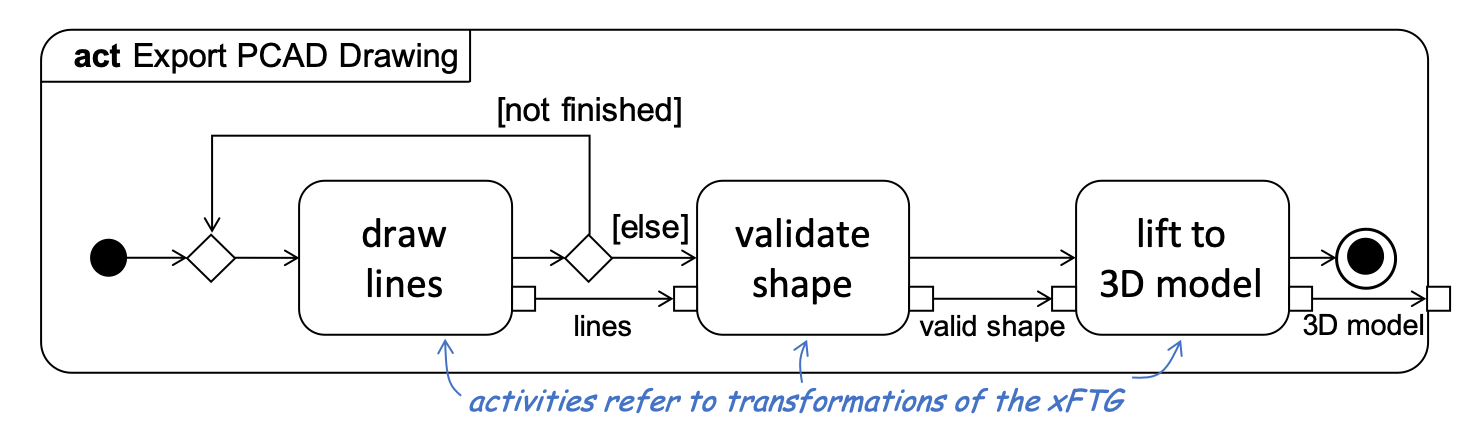
\includegraphics[width=0.98\columnwidth]{process}
\vspace{-1em}
\caption{A process model for \textsc{CCad} that yields a valid shape and
   creates a 3D cookie cutter shape from it.} 
\label{fig:Process}%
\end{figure}

%%
We may distinguish in the concrete syntax $\mathsf{ControlFlow}$s from 
$\mathsf{ObjectFlow}$s to emphasize the control and make the process more 
prominent. 
We assume that $\mathsf{ActionNode}$ names and $\mathsf{ObjectNode}$ names 
are distinct and unique. We also require that \textsc{Pm}s are well-formed 
wrt. their \textsc{Ftg}.

Notice that our definition for x\textsc{Ftg}s relies solely on \emph{names}: a 
framework should take care of retrieving the actual transformation item (as per 
Def. \ref{def:Transformation}) from the transformation name (trough 
the $trans$ of Def. \ref{def:Naming}), and should check that the language 
instances used as object nodes conform to languages that actually implement the 
abstract formalisms or languages (through $form$ and $lang$) mapped to that 
transformation name in the appropriate 
order.

\medskip
The following definition simply puts things together: a workflow is composed of 
an \textsc{Ftg} together with several well-typed \textsc{Pm}s. 

%%%%%%%%%%%%%%%%%%%%
% WORKFLOW
%%%%%%%%%%%%%%%%%%%%
\andreas{Shouldn't the following defintion use xFTG?}
\begin{Definition}[\label{def:Workflow}Workflow]
   A \emph{workflow} $\mathsf{W}\in\mathbb{W}(FL, T)$ is a pair $\mathsf{W} = 
(\mathsf{FTG}, \mathsf{P})$ where $\mathsf{FTG}\in\FTG(FL, T)$ and 
$\mathsf{P}\in\wp(\PM)$, such that $\mathsf{P}$ is well-formed (noted 
$\mathsf{P} \blacktriangleright \mathsf{FTG}$) wrt. $\mathsf{FTG}$, i.e. for 
each $\mathsf{ActionNode}$ inside $\mathsf{P}$ with name 
$tn\in\mathsf{TransInstance}$,
\begin{itemize}
   \item $tn$ is explicitly typed by a transformation (name) captured in the 
domain of $\mathsf{FTG}$ (i.e. $type(tn) = t \in \Dom{\mathsf{FTG}}$);

   \item for each source or target $fl_i$ of $t$ at rank $i$, there exists a 
$\mathsf{Pin}$ at rank $i$ connected (as input or output) to an 
$\mathsf{ObjectNode}$ carrying an object (instance) $\mathsf{LI}\in 
\mathsf{LangInstance}$ typed by a language $\mathsf{L}\in\mathbb{L}$, such that 
$\mathsf{LI} \;\rhd\; \mathsf{L}$, and $\mathsf{L}\rightsquigarrow F$, then one 
of the following holds:
   \begin{itemize}
      \item $fl_i\in \mathsf{AbstractFormalismN}$ then $fl_i$ denotes an 
abstract formalism that should refine (some 
of) the formalisms implemented by $\mathsf{L}$, i.e. $form(fl_i) \sqsubseteq 
\mathsf{F'_{k_1}}, \ldots form(fl_i) \sqsubseteq \mathsf{F'_{k_n}}$ such that 
$\mathsf{F'_{k_1}}, \ldots \mathsf{F'_{k_n}} \subseteq F$;
      
      \item $fl_i\in \mathsf{LanguageN}$ then $fl_i$ denotes a language. The 
language that should refine $\mathsf{L}$ i.e. $lang(fl_i) \sqsubseteq 
\mathsf{L}$.
   \end{itemize}
\end{itemize}
\end{Definition}
\noindent
When clear from context, or unnecessarily detailed, we simply note the set of 
workflows $\mathbb{W}$, without any indication of languages or 
transformations (sets).

Similar to the original  
\cite{Mustafiz-etAl:2012,Lucio-Mustafiz-etAl:2013,TR:Lucio-Mustafiz-etAl:2012},
our definition does not impose a particular topology on the $\mathsf{PM}$ as 
long as transformations are well-formed. However, the original definition 
simply rely on a name-matching typing: a transformation (resp. language) 
instance in a $\mathsf{PM}$ is denoted using \UML's Object notation for names, 
say $\mathsf{:Trans}$, that need to match an existing transformation (name) 
$\mathsf{Trans}$ in $\mathsf{FTG}$. In constrast, we relaxed this matching 
process by allowing ''template`` transformations based on abstract formalisms 
that capture the main concepts manipulated by a transformation, which imposes 
to rely on the two relations of Def. \ref{def:Implementation} (implementation 
and refinement). Similar to substitution for object-oriented methods, this 
paves the way to more intensive reuse of transformation ''templates'' at the 
expense of checking that the refinement relations hold.

\begin{Example}[\label{ex:TBA}\textsc{Pcad} Workflow]
   Figure \ref{fig:PCAD-FTG} depicts an \textsc{Ftg} for \textsc{Cad} with 7 
transformations that have the abstract formalism $\mathsf{Product}$ as source, 
target or both. For example, an iterative process may instantiate 
$\mathsf{Create}$, $\mathsf{Modify}$ and $\mathsf{isValid}$ to produce a target 
$\mathsf{Product}$ that is guaranteed to be always valid.  

%\begin{figure}[t]
%   \centering
%   \includegraphics[width=0.98\columnwidth]{PCAD-FTG+PM}
%   \caption{A possible workflow $\mathsf{W_{PCAD}} = (\mathsf{FTG_{PCAD}}, 
%\mathsf{PM_{PCAD}})$, with the x\textsc{Ftg} on the left and the \textsc{Pm} 
%on the right}%
%   \label{fig:PCAD-MM}%
%\end{figure}

\begin{figure}[t]
   \centering
   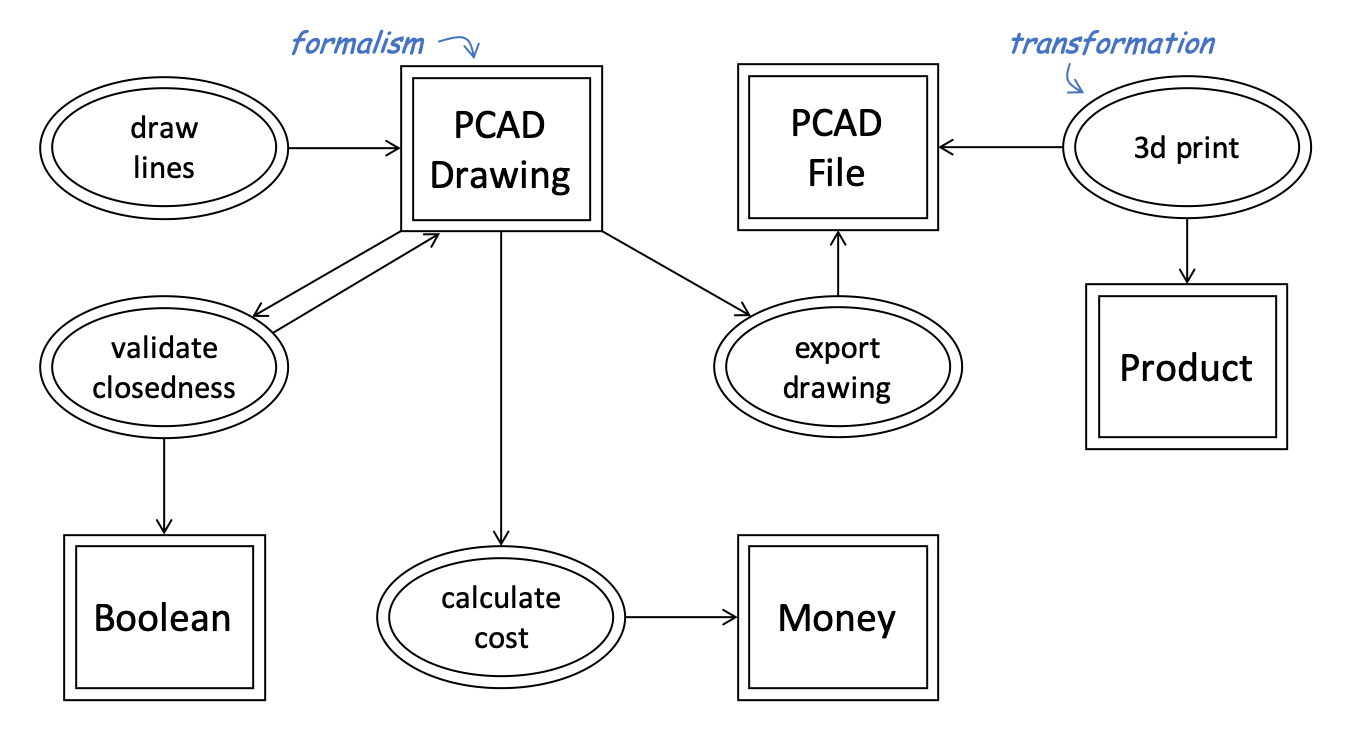
\includegraphics[width=0.98\columnwidth]{FTG}
   \caption{x\textsc{Ftg} of a possible workflow $\mathsf{W_{PCAD}} = (\mathsf{FTG_{PCAD}}, 
\mathsf{PM_{PCAD}})$ that supports the process model of Fig.~\ref{fig:Process}.}%
   \label{fig:PCAD-MM}%
\end{figure}

\end{Example}

%%%%%%%%%%%%%%%%%%%%%%%%%%%%%%%%%%%%%%%%%%%%%%%%%%%%%%%%%%%%%%%%%%%%%%%%%%%%
\subsection{Paradigm}
\label{sec:PS}

From our viewpoint, a paradigm is a set of properties that captures 
certain specific characteristics that shall hold over languages and/or 
processes. To simplify the checking, we define a \emph{paradigmatic structure} 
as a potential candidate holding a particular paradigm.

%%%%%%%%%%%%%%%%%%%%
% PARAD. STRUCTURE
%%%%%%%%%%%%%%%%%%%%

\begin{Definition}[Paradigmatic Structure]
   A \emph{paradigmatic structure} $\mathsf{PS}\in \PS$ is a pair $\mathsf{PS} 
= (L, W)$ where $L\in \wp(\mathbb{L})$ is a set of languages and 
$W \in \wp(\mathbb{W})$ is a set of workflows.
\end{Definition}

Table \ref{tab:Properties} already described some interesting properties 
related to three well-known paradigms. As easily noticeable, properties span 
over all elements constituting a paradigmatic structure: the components of the 
languages involved (and potentially, properties that require certain 
combinations of languages); transformations; and also the processes. Some 
paradigms may also have ''sanity-check`` properties that characterise the 
paradigm itself. We will call these properties capturing the essence of a 
paradigm \emph{paradigmatic properties}.

Following the mantra of modelling ''at the most appropriate 
level of abstraction``, it becomes impossible at the abstraction level of this 
presentation to formally (i.e., intensionally) define the nature of such a large 
class of properties. We therefore provide an extensional definition: we note 
$\mathcal{P}(S)$ the set of all possible properties expressible over a 
structure $S$. 

%%%%%%%%%%%%%%%%%%% 
% PARAD. PROPERTIES 
%%%%%%%%%%%%%%%%%%%

\begin{Definition}[\label{def:ParaProperties}Paradigmatic Properties]
   A \emph{paradigmatic property} is a tuple
$\pi = (\pi_{\mathsf{L}},\pi_{\mathsf{W}},\pi_{\mathsf{PS}}) \in \Pi$ where
\begin{itemize}
   \item $\pi_{\mathsf{L}} \in \mathcal{P}(\mathbb{L})$ is a set of properties 
over languages;
   \item $\pi_{\mathsf{W}} \in \mathcal{P}(\mathbb{W})$ is a set of properties 
over workflows;
   \item $\pi_{\mathsf{PS}}\in\mathcal{P}(\PS)$ is a set of 
properties spanning over all components of paradigmatic structures).
\end{itemize}
\end{Definition}
\noindent
Paradigmatic properties may be expressed through \emph{pattern languages}, e.g., 
for ensuring the presence of certain concepts, or through \emph{dedicated 
logics}, e.g., for ensuring semantic properties. We detail later in the examples 
how some properties described in Table \ref{tab:Properties} may be captured 
precisely.

For instance, relevant paradigmatic properties for a paradigmatic structures $PS
= \left(L,W\right)$ representing Simple Computer Aided Design in the sense of
Table~\ref{tab:Properties}, $\Pi_{SCAD}$, could be
\begin{itemize}
%%
\item $\pi_{\mathsf{SCAD1}} \equiv$ $L$ features a class $P$ that has two 
attributes $a$ and $b$ that each support values of $\mathbb{R}$ and a class $L$ 
that has two instances of $P$. 
%%
\item $\pi_{\mathsf{SCAD2}} \equiv$ $L$ features a class $D$ that captures a 
collection of $L$ instances; 
 
\item $\pi_{\mathsf{SCAD3}} \equiv$ $W$ supports translating $D$ instances into products;
% \item $\pi_{\mathsf{W_2}}...$ there is a workflow that supports checking
% closedness of shapes.
\end{itemize}

\label{fig:LanguageProperties} illustrates $\pi_{\mathsf{CAD1}}$ and
$\pi_{\mathsf{CAD2}}$ as patterns over the abstract syntax of $L$. These
patterns could be modeled and matched leveraging the notion of model
types~\cite{steel2007model}, which ultimately checks conformance as graph
isomorphism between the two metamodels (out of which one would be the pattern).
The representation of $\pi_{\mathsf{CAD3}}$ depends on the representation of the
xFTG. Generally, this entails that the xFTG of $W$ of the $PS$ must comprise a
sequence of formalisms and transformations that begins with the formalism $D$
matched for representing drawings and ends with a formalism representing
products. 

\begin{figure}[t]
   \centering 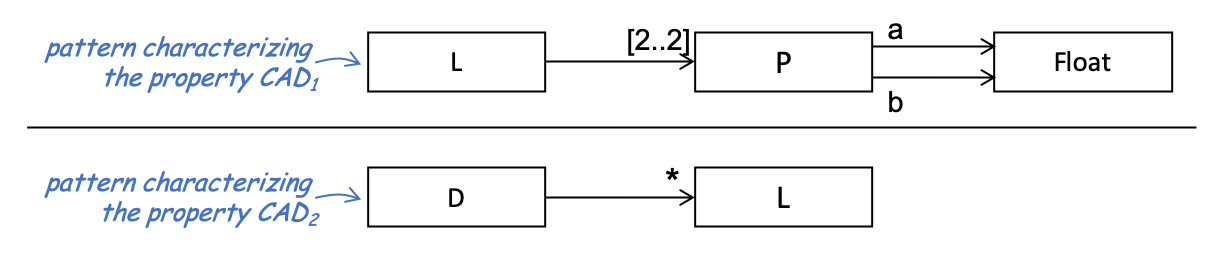
\includegraphics[width=\columnwidth]{LanguageProperties.png}
   \caption{Patterns characterizing two paradigmatic properties over the abstract 
   syntax of the language of a paradigmatic structure.}  
   \vspace{-1em}
   \label{fig:LanguageProperties}
\end{figure}


%%%%%%%%%%%%%%%%%%%%
% INTENT
%%%%%%%%%%%%%%%%%%%%

\begin{Definition}{\label{def:Paradigm}Intent --- Paradigm}
We define an \emph{intent} $\iota$ as a \emph{named} paradigmatic property, 
i.e., $\iota \in [\mathsf{IntentN} \to \Pi]$.

   Let $\mathsf{PS} = (L, W)\in\PS$ be a paradigmatic structure and 
$\mathsf{p}$ an intent (name) captured by a predefined $\iota$ (i.e., 
$\mathsf{p}\in \mathsf{Dom}(\iota)$ such that 
$\iota(\mathsf{p}) = (\pi_{\mathsf{L}}(\mathsf{p}), 
                     \pi_{\mathsf{W}}(\mathsf{p}), 
                     \pi_{\mathsf{PS}}(\mathsf{p}))$). 
$\mathsf{PS}$ is said to \emph{embody} $\mathsf{p}$ (alternatively, 
$\mathsf{PS}$ \emph{follows} $\mathsf{p}$) iff 
\begin{itemize}
   \item the properties $\pi_{\mathsf{L}}(\mathsf{p})$ hold on $L$;
   \item the properties $\pi_{\mathsf{W}}(\mathsf{p})$ hold on $W$; and
   \item the properties $ \pi_{\mathsf{PS}}(\mathsf{p}))$ hold on $\mathsf{PS}$.
\end{itemize}
\end{Definition}

\begin{Example}[PCAD Properties on Cost]
   \moussa{Review example from Workshop!}
\end{Example}

Following this definition, it is obvious that the paradigmatic properties of
$\Pi_{CAD}$, hold for our exemplary \CCad paradigmatic structure sketched by the
formalism of Def.~\ref{def:CCAD} and the metamodel depicted in
Fig.~\ref{fig:PCAD-MM}:
% %
\begin{inparaenum}[(1)]
% %
\item For the first syntactic property $\pi_{\mathsf{SCAD1}}$, we can match
class $P$ to Point, $a,b$ to $x,y$, and $L$ to Line;
% %
\item For the second syntactic property $\pi_{\mathsf{SCAD2}}$, we can match
class $D$ to class CCAD; and
% %
\item For the workflow property $\pi_{\mathsf{SCAD3}}$, we ca the sequence of
transformations starting with formalism ``CCAD Drawing'' that transforms it into
an ``3D Model'' and afterwards into a ``Product'' in its xFTG.
\end{inparaenum}
Hence, we can establish that the paradigmatic structure sketched by \CCad
embodies (or follows) the SCAD formalism.


